%\documentclass[11pt]{beamer}
\documentclass[11pt,handout]{beamer}

\usepackage{amsmath, graphicx, natbib, verbatim, color}
\usepackage{colortbl}
%\usetheme{CambridgeUS}

\useoutertheme{infolines}
\usetheme{default}

\setbeamertemplate{navigation symbols}{}
\setbeamertemplate{headline}{}
\setbeamertemplate{itemize items}[circle]
\usefonttheme{serif}
\usepackage{palatino}

%\setbeamercolor{title}{bg=black!20!white}
%\setbeamercolor{frametitle}{bg=black!20!white}
%\setbeamercolor{alerted text}{fg=red!100!white}
%\setbeamertemplate{blocks}[rounded][shadow=true]

\setlength{\itemsep}{1.5ex}
\setlength{\parskip}{1.5ex}



\setbeamertemplate{navigation symbols}{}
\AtBeginSection[]
{
   \begin{frame}
       \frametitle{The Thread}
       \tableofcontents[currentsection]
   \end{frame}
}



\definecolor{forest}{rgb}{.15, .5, .15}
\definecolor{brick}{rgb}{.7, .15, .15}
\definecolor{darkgreen}{rgb}{.15, .5, .15}
\definecolor{darkred}{rgb}{.7, .15, .15}
\definecolor{darkblue}{rgb}{.15, .15, .7}
\definecolor{Green}{rgb}{0.2,1,0.2}

\usepackage[english]{babel}
\usepackage[latin1]{inputenc}
\usepackage{times}
\usepackage[T1]{fontenc}

\setlength{\itemsep}{15em}


\title[CanCORS]% (optional, with long titles)
{Cancer Care Outcomes Research and Surveillance Consortium \\
(CanCORS) \\ \vspace{0.4in}
Using Multiple Imputation to both Uncover and Hide}

\author[Harrington]{Dave Harrington (\texttt{dph@jimmy.harvard.edu}) }


\institute % (optional)
[DFCI/Harvard] {{\color{darkgreen} Dana-Farber Cancer Institute, Harvard Statistics and Biostatistics}}

\date{10 June 2014}

\setbeamertemplate{navigation symbols}{}

\begin{document}



\begin{frame}

  \titlepage

\end{frame}

\begin{frame}{Collaborators}

Alan Zaslavsky, HMS \\
\medskip
Yulei He, CDC \\
\medskip
Bronwyn Loong, Australian National University \\
\medskip
Paul Catalano, DFCI and HSPH \\
\medskip
MaryBeth Landrum, HMS \\
\medskip
Many members of the CanCORS Consortium

	
\end{frame}

\begin{frame}{Outline \dots}
\tableofcontents
\end{frame}


\section{Brief Overview of CanCORS}

\begin{frame}[plain]

\begin{center}
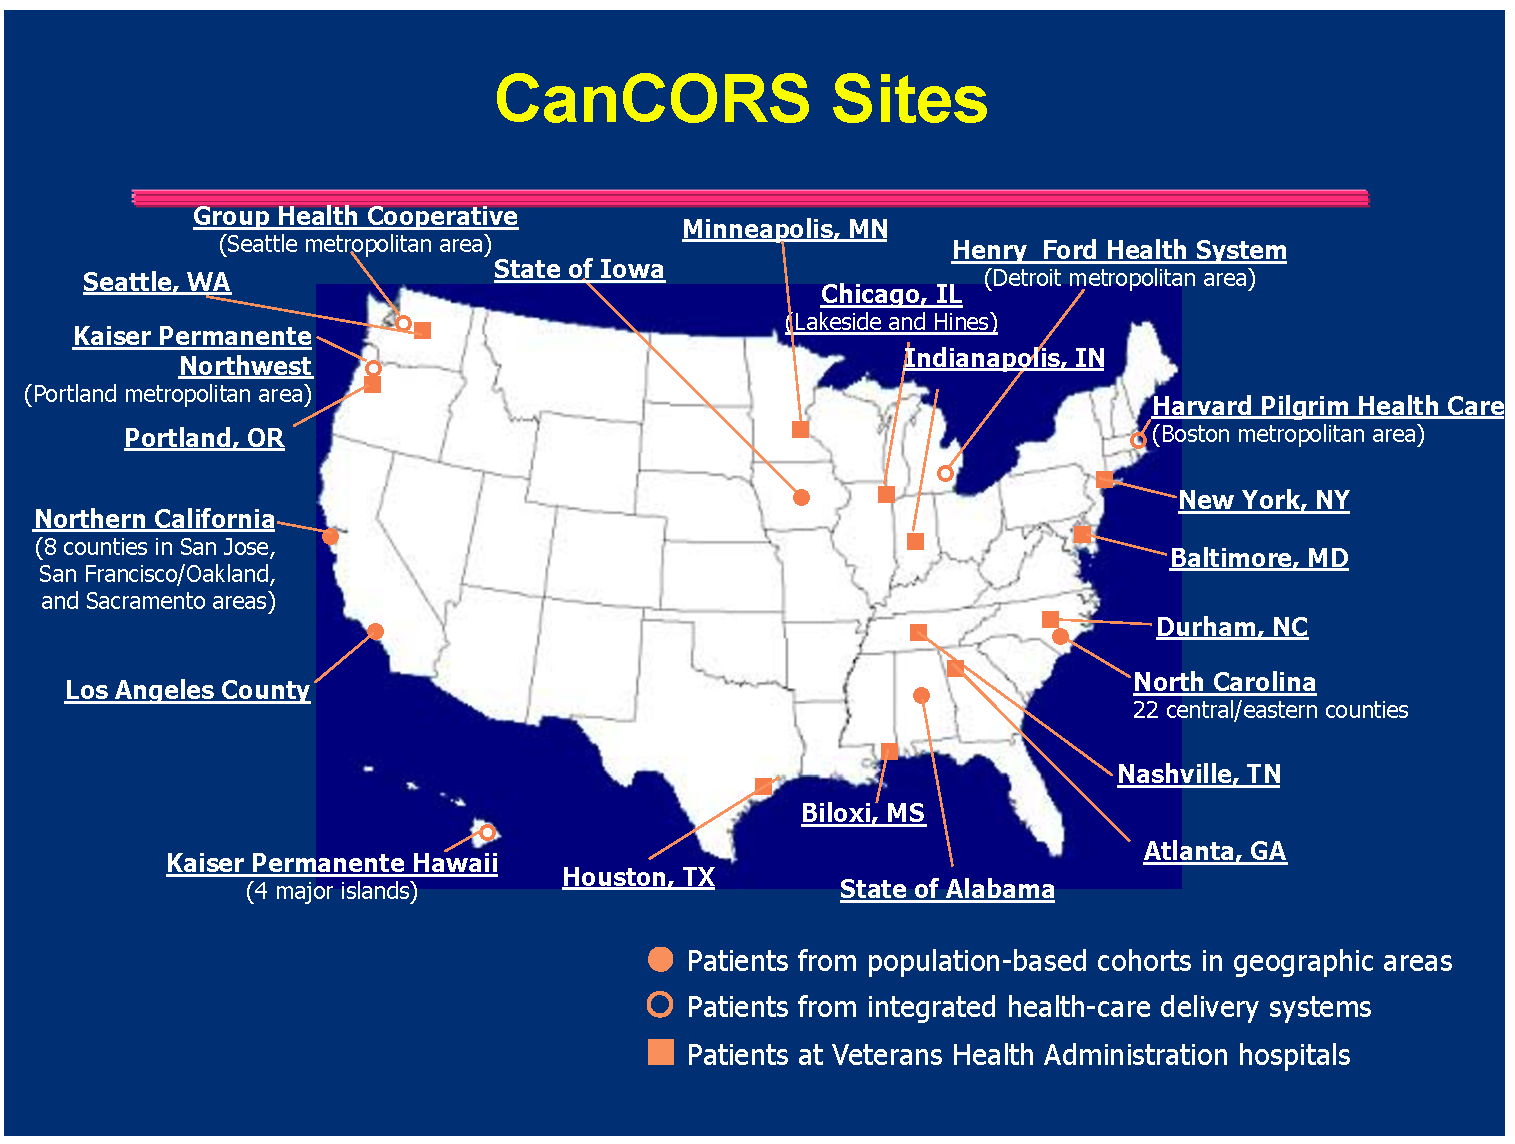
\includegraphics[width= 1.0\textwidth]{./figures/cancors_sites.pdf}
\end{center}

\end{frame}


\begin{frame}{}

\begin{center}
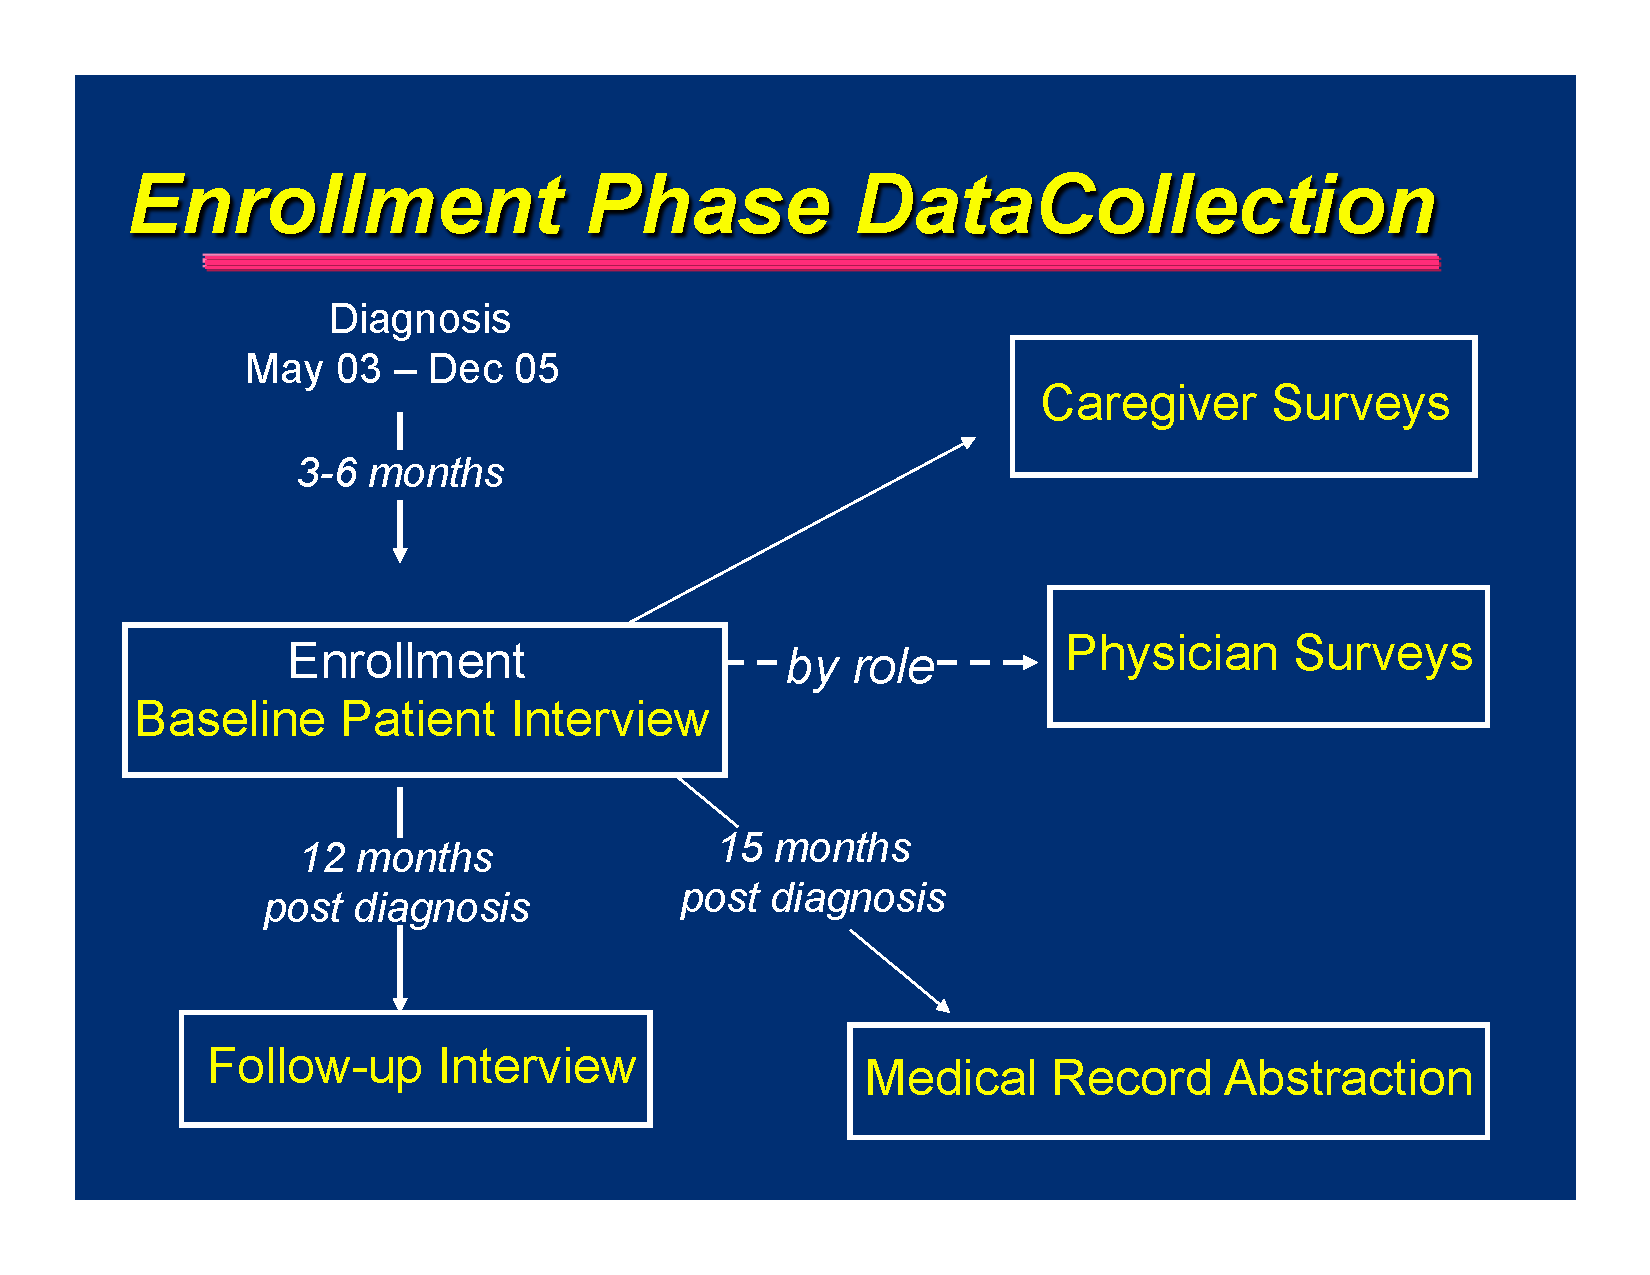
\includegraphics[width= 1.0\textwidth]{./figures/initial_instruments.pdf}
\end{center}

\end{frame}

\begin{frame}{Interview Instrument Types}

\begin{itemize}

  \item Full baseline 
  
  \medskip
  
  \item Brief baseline
  
  \medskip
  
  \item Surrogate living and decedent

\end{itemize}
	
\end{frame}



\begin{frame}{}

\begin{center}
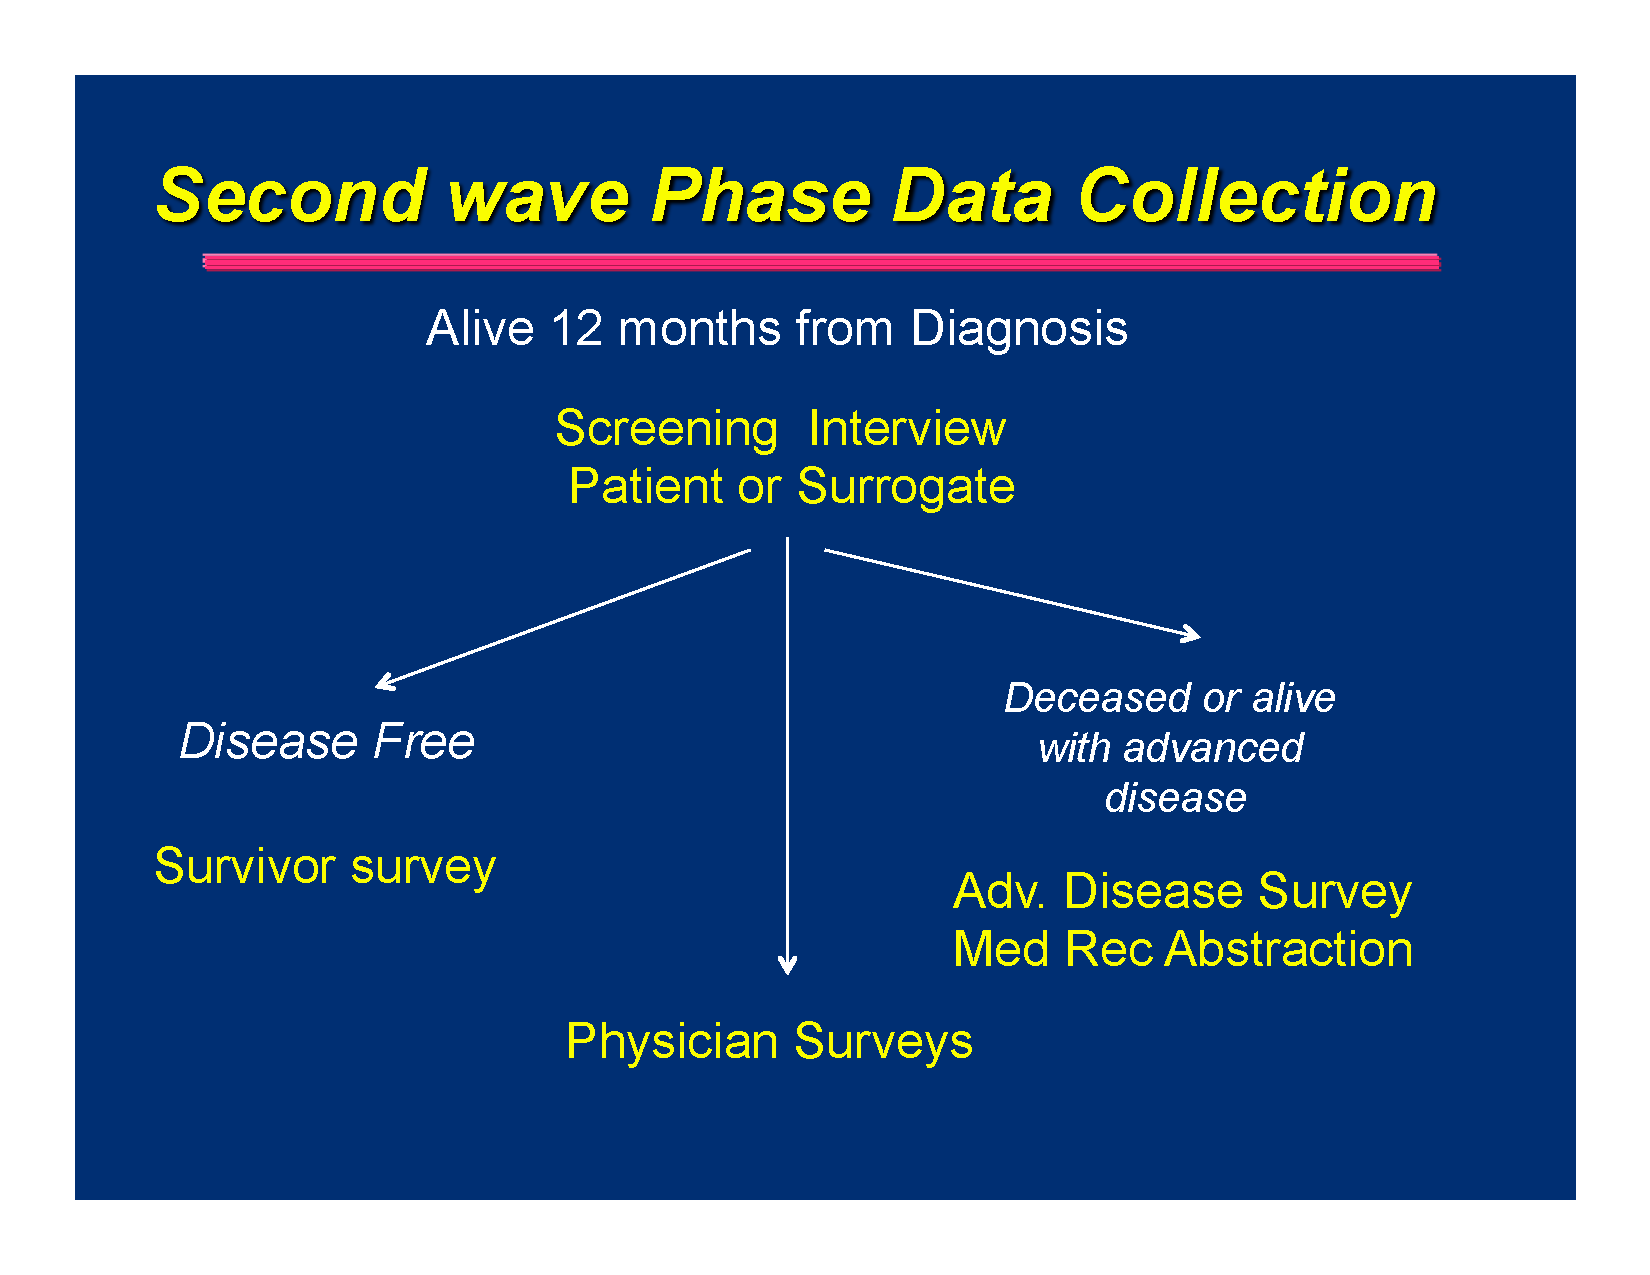
\includegraphics[width= 1.0\textwidth]{./figures/second_wave.pdf}
\end{center}

\end{frame}

\begin{frame}{Enrollment}

10,061 patients with lung or colorectal cancer enrolled, with data from	

\begin{itemize}

  \item Patient interviews

  \item Physician surveys

  \item Medical record abstraction

\end{itemize}

  2,995 patients recontacted in second wave
   
  \begin{itemize}
  
   \item Revisions of earlier instruments

   \item Assessing recurrence surveillance using electronic records in
   integrated health plans and Medicare Claims

   \end{itemize}

\end{frame}


\begin{frame}{}

\begin{center}
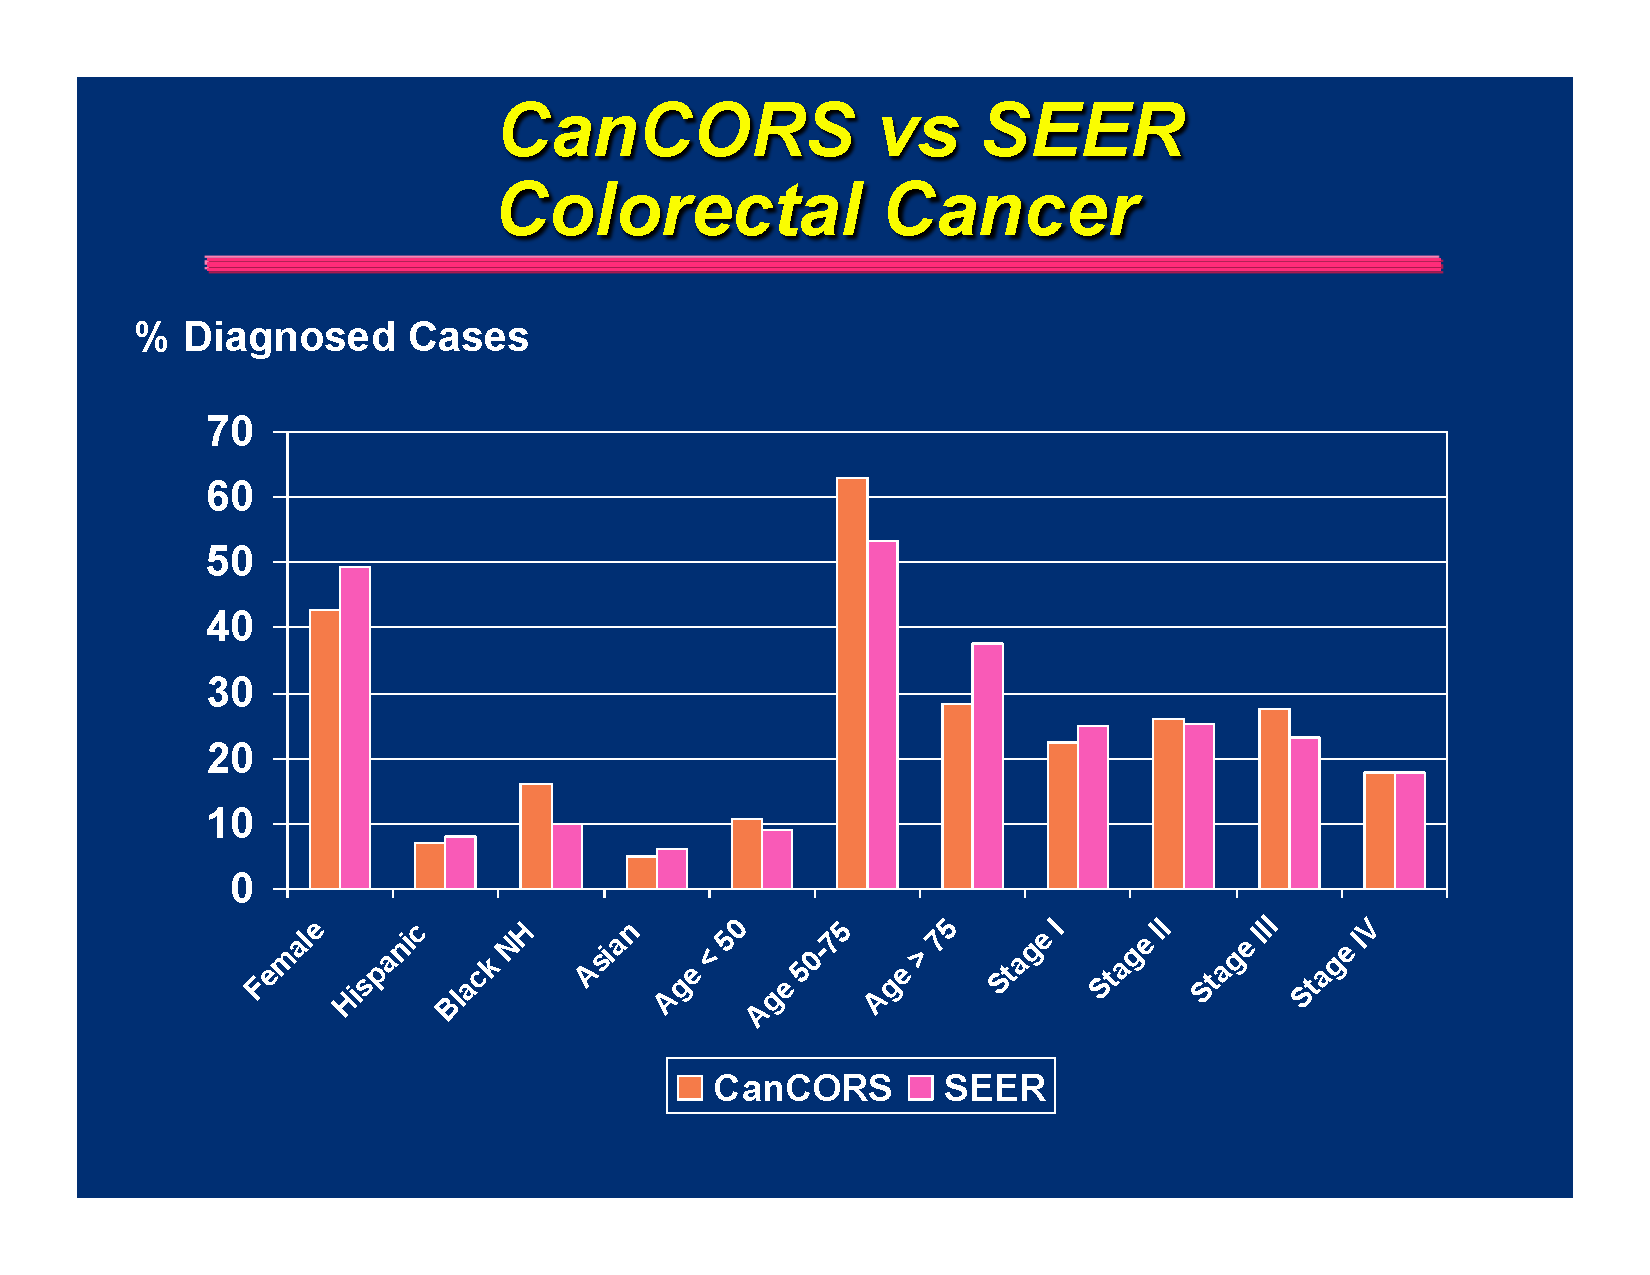
\includegraphics[width= 0.9\textwidth]{./figures/cancors_seer_crc.pdf}
\end{center}

(Catalano, \textsl{Med Care}, 2012)
\end{frame}


\begin{frame}{Challenges in the Design and Analysis}

  \begin{itemize}
     
     \item Uniform data collection/standards of analysis
     
     \medskip
     
     \item Unit non-response
     
     \medskip
     
     \item \textcolor{forest}{Item non-response}
     
     \medskip
     
     \item \textcolor{forest}{Confidentiality}
  \end{itemize}


\end{frame}

\section{Multiple Imputation (MI) Primer}
 

\begin{frame}{Multiple Imputation}

Proposed by Rubin in 1977; Rubin's 1996 JASA review is accessible.

\begin{itemize}

   \item Schafer 1999 SMMR paper is a primer


   \item Multiple draws (usually 5 - 10) used to create versions of completed dataset.

\begin{itemize}
   \normalsize
   \item Draws taken from posterior predictive distribution of missing data, given observed data.

\end{itemize}


   \item Each dataset analyzed using traditional complete case analysis.


  \item Variance estimates account for within and between imputation variability.
  
\end{itemize}
	
\end{frame}

\begin{comment}

\begin{frame}{Use in health care research}

Used in 

\begin{itemize}

  \item NHANES III (1992 - 1993)
  
  \item Analysis of Milwaukee School Voucher Program

\end{itemize}
	
\end{frame}

\end{comment}
 
\section{Unit Non-response: Using MI to `uncover'}


\begin{frame}{Missingness in the surveys}

\begin{center}
\begin{scriptsize}
   \begin{tabular*}{0.85\textwidth}{@{\extracolsep{\fill}} lllllll}
   \hline
   {Survey} & {No. Vars} & {Sample Size} & 
   \multicolumn{2}{c}{{Skips(\%)}} & 
   \multicolumn{2}{c}{{DO/DK/REF(\%)}} \\
   & & & & & & \\
   & & & Mean & Range & Mean & Range \\ 
   & & & & & &  \\ \hline
   & & & & & & \\
   Full Baseline & 535 & 5763 & 50 & 0-99 & 1.23 & 0-37 \\   
   Brief Baseline & 156 & 1397 & 48 & 0-99 & 2.49 & 0-22 \\
   Surrogate Live & 413 & 1083 & 50 & 0-99 & 1.61 & 0-28 \\
   Surrogate Deceased & 473 & 1827 & 62 & 0-99 & 1.46 & 0-29 \\
   Follow-up & 384 & 6087 & 65 & 0-99 & 0.55 & 0-33 \\ 
   \end{tabular*}
\vspace{0.2in}
	
DO/DK/REF = Drop Out/Don't Know/Refused	
\medskip

\end{scriptsize}
\end{center}

Some complete case analyses drop approximately 30\% of respondents.
	
\end{frame}

\begin{frame}{Challenges to MI}

	
\begin{itemize}

  \item Several different data types
  
  \item 4 instruments used in two cancer types
  
  \item Block missingness because of missing domains in shorter surveys.
  
  \item Extensive skip patterns in interview structure
  
  \item Data set periodically refreshed
  
  \item Diagnostics difficult

\end{itemize}
	
\end{frame}


\begin{frame}{Imputation Strategy}

  \begin{itemize}
     
     \item Use Sequential Regression Multiple Imputation (SRMI), implemented in SAS module IVEWare. (Raghunathan, 2001, \textsl{Surv. Meth})
     
     \item Imputation used to create 5 datasets for each of the two cancer types.
     
     \item Within a cancer, imputation based on dataset with instrument types combined.
     
     \item Skipped questions and missing blocks in shorter surveys imputed
     
     \item Skips and block missingness restored after imputation
     
     \item To incease \textsl{congeniality}, imputation did not use data available to Coordinating Center but not available to data analysts.
     
  \end{itemize}

	
\end{frame}

\begin{frame}{Diagnostics}

\begin{itemize}

  \item Examined changes in marginal means, pairwise correlation coefficients.

  \item Comparisons with complete case and missingness indicator analyses.
  
  \item Comparisons with weighted analyses: treat brief/surrogate surveys as item non-response, non-response weights calculated for participation in full survey.
  
% \item Posterior predictive $p$-values.

\end{itemize}
	
\end{frame}


\begin{frame}{Comparative Analyses of Hospice}
	
	Full analysis in Huskamp, et al., Arch Int Med (2009)
	
	Did you participate in a discussion of hospice with your physician?
	
	\begin{center}
	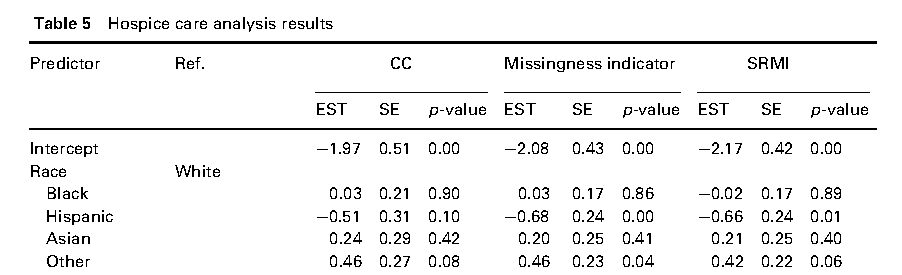
\includegraphics[width= 1.0\textwidth]{./figures/table_5.pdf}
	\end{center}

	Table is small piece of full logistic regression.
	
	Complete account in He, et al. 2010, \textsl{SMMR}
	
\end{frame}


\begin{frame}{Weighted analyses: QoL scores}
	
	\begin{center}
	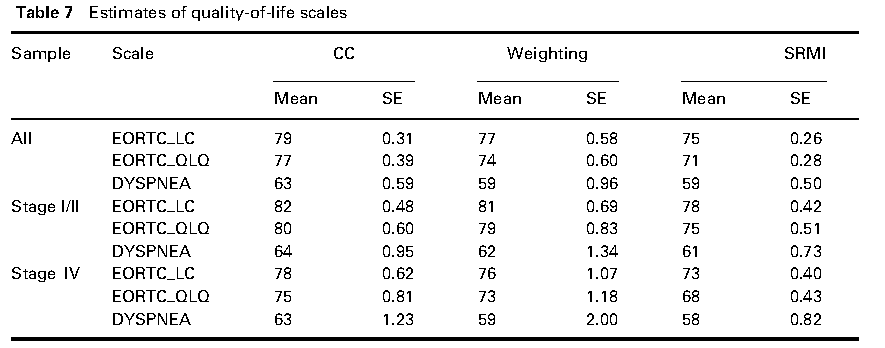
\includegraphics[width= 1.0\textwidth]{./figures/qol_diagnostic.pdf}
	\end{center}
	
	
\end{frame}




\section{Confidentiality: Using MI to Hide}

\begin{frame}
\frametitle{Challenges in preserving confidentiality with publicly available healthcare microdata}

\begin{itemize}


\item Minimize disclosure risk. 

\begin{itemize}

  \normalsize
  
  \item Reduce risk of participant re-identification by malicious user should be acceptably low.

\end{itemize}
\medskip


\item Maintain data utility.

\begin{itemize}

  \normalsize
  
  \item Modifications to the observed data set should maintain variable relationships that are both clinically plausible and reproduce (approximately) relationships in the data.
 
\end{itemize}


\item Low maintenance for Coordinating Center

\end{itemize}

\end{frame}

\begin{frame}
\frametitle{Background on partially synthetic data}

\textbf{Idea:} Replace the observed values for sensitive variables or key identifiers with synthetic data.  Do not release original values of these variables.

\begin{itemize}

\item First proposed by Rubin (1993) based on the concepts of multiple imputation.

\item Synthetic values are created using samples drawn from the posterior predictive distribution  of target population responses given the observed data set.

\item Analysts can draw approximately valid inferences
about the target population of interest using standard methods for multiply imputed data.


\end{itemize}


\end{frame}


\begin{frame}
\frametitle{Synthetic data in practice}

\begin{itemize}
\item Survey of Consumer Finances
\item American Communities Survey
\item Survey of Income and Program Participation
\item US Longitudinal Business Database
\item Longitudinal Employer - Household Dynamics
\item German IAB Establishment Panel 
\end{itemize}

\end{frame}

\begin{frame}
\frametitle{Identification of variables to synthesize}

\begin{itemize}

\item \textbf{Direct identifiers:} name, postal address, SSN: not available to internal and external investigators, so not synthesized.

  \medskip
  
\item \textbf{Quasi-identifiers:} Age, education, sex, marital status, race. 

\medskip

\item \textbf{Clinical:} Not synthesized; complex structure - difficult to synthesize, accessible by insiders only (not wider population); subject to judgemental variation and incomplete medical record acquisition

\medskip

\item \textbf{Sensitive:} All information gathered can be considered sensitive; full synthesis not practical and not useful to data analysts

\end{itemize}

Details reported in Loong, et al. (2013) \textsl{Stat. Med.}


\end{frame}

\begin{frame}
\frametitle{Imputation models}

\begin{equation}
f(Y^{\mathrm{(j)}}_{\mathrm{age}},Y^{\mathrm{(j)}}_{\mathrm{educ}},Y^{\mathrm{(j)}}_{\mathrm{marstat}},Y^{\mathrm{(j)}}_{\mathrm{race}},Y^{\mathrm{(j)}}_{\mathrm{sex}} \big | Y_0, \mathbf{S}_0) \ ,
\label{eq:jmpost}
\end{equation}

Not practical to draw directly from conditional joint distribution of identifiers, given observed data.


\smallskip

We used sequential regression multiple imputation here as well


\smallskip

Parametric approach to imputation  - logisitic regression model to impute sex, multinomial logit models for other variables.

\smallskip
$m$ = 5 partially synthetic data sets created 
\smallskip

Imputations done in \textsf{R} package \textsl{MI} for this project.  

\end{frame}

\begin{frame}
\frametitle{Imputation models}

\begin{itemize}
\item Select predictor variables using stepwise regression within each of 12 sections of survey.
\item On average $\approx$ 50 predictors for each variable to be imputed.

\item No interactions, main effects only - reduce risk of overfitting (which increases disclosure risk), reduce computational burden and avoid multicollinearity and separation issues.  

\item Variables included in all imputation models: survey disposition code, stage, histology, vital status, study site.

\end{itemize}

\end{frame}


\begin{frame}
\frametitle{Disclosure risk}

\begin{itemize}

\item \textbf{Identification disclosure risk}: potential identification of sampled units in the released data

\medskip

\item \textbf{Inferential disclosure risk}: inference of new information about a known participant in the survey, e.g., all participants with the same identifiers have the same income.

\end{itemize}

Inferential disclosure risk a difficult problem, that is still not well-understood.
We focus on identification disclosure risk assessment.  

\end{frame}

\begin{frame}
\frametitle{Identification disclosure risk assessment}

Duncan and Lambert and risk framework (1989)

\begin{itemize}

\item Mimic the behavior of an ill-intentioned public user (an intruder)
who has the true values of unique or quasi-identifiers for select target units and wants to identify the records in the synthetic data that have matching identifier values.

\item We investigated 3 sets of quasi-identifying values representing varying assumed levels of intruder information\\
(i) Set 1: Age, sex, marital status, and race \\
\textcolor{forest}{(ii) Set 2: Set 1 + education + income level} \\
(iii) Set 3: Set 2 + disease stage + study site \\
\end{itemize}

\end{frame}

\begin{frame}
\frametitle{Identification disclosure risk assessment}

A potential identification risk for target record $i$ occurs when its quasi-identifying values match the corresponding values for a record $k$ in synthetic data set $j$.
 
\medskip

Some assumptions/definitions about risk of identification:
\begin{itemize}

\item The intruder knows the target is in the survey and the quasi-identifiers of all units in the population.

\item If target record has no matching quasi-identifiers among the $m$ imputed data sets, risk of identification is zero.

\item  Expected match risk: probability of correct match if intruder randomly guesses the match from the candidates with same quasi-identifiers

\item Maximum match risk: intruder correctly always correctly identifies record from among potential candidates

\item Total match risk: probability that a record is correctly \textsl{and} uniquely identified in synthetic data.

\end{itemize}



\end{frame}

\begin{comment}

Outline disclosure risk in a special case.  Pick second set of
quasi-identifiers, build up intuition for EMR.

  -- Assumptions about the behavior of an intruder
     -- If an intruder has a record  with true values of quasi-identifier, he/she 
     searches the data set for a match.  With synthetic data, searches
     all data sets.
     
     -- If more than one match, pick one randomly
     
  -- Disclosure risk is expected fraction of cases in data set where imputer 
  guesses correctly
  
  -- Worse case: a subject has a correct match, intruder always guesses correctly.
  
  -- What is the reduction in disclosure risk
  
  -- Give quasi-identifiers,  talk through what is happening.
  
  

\end{comment}}


\begin{frame}
\frametitle{Disclosure risk \ldots}

Compute probabilities of identification under three sets of quasi-identifiers.

\vspace{0.1in}

\begin{itemize}
\item[(i)] \textit{Set 1}:  Age, sex, marital status, race

\medskip

\item[(ii)] \textit{Set 2}:  \textcolor{forest}{Set 1 + income level + education}

\medskip

\item[(iii)] \textit{Set 3}: Set 2 + disease stage +  PDCRID

\end{itemize}
 
\end{frame}

\begin{frame}
\frametitle{Disclosure risk estimates, lung cancer cohort}

Using Set 2 of identifiers:

Synthetic data:

\begin{itemize}

  \item Expected match risk: 217/5000 = 4.3\%
  
  \item Maximum risk: 925/5000 = 18.5\%
  
  \item Total match risk: 88/5000 = 1.7\%

\end{itemize}

Observed data:

\begin{itemize}

  \item Expected match risk: 1770/5000 = 35.4\%
  
  \item Maximum risk: 5000/5000 = 100\%
  
  \item Total match risk: 989/5000 = 19.8\%

\end{itemize}

\end{frame}

\begin{frame}{Calculating disclosure risk}

Expected match rate, identifier set 2, lung cancer:

\begin{itemize}

  \item \textsl{Total Match Risk}: 88 cases where original record correctly and uniquely matched to synthetic data record.
  
  \item \textsl{Maximum risk}:  1158 instances where a true record was among identical sets of identifiers in 5 synthetic data sets.  Corresponds to 958 unique records
  
  \item \textsl{Expected matches:} Expected number of matches if intruder guessed randomly among potential set of matches.  This is a weighted average first within then across synthetic data sets.


\end{itemize}

\end{frame}



\begin{frame}{Disclosure risk by set of indentifiers}

\begin{table}[!h]
\caption{\emph{Disclosure risk  - CanCORS lung cancer \textbf{partially synthetic} data}}
\centering
\begin{tabular}{lllll}   
\textbf{Quasi-identifier set} & \multicolumn{2}{c}{\textbf{EMR}} & \multicolumn{2}{c}{\textbf{TMR}}  \\  \hline
  &  Obs. & Syn. &  Obs. & Syn. \\ 
1 &  70 & 38 & 0 & 0  \\ 
2 &  1770 & 217 & 989 & 88\\
3  & 4495 & 890 & 4000 & 717 \\  
\end{tabular}

\label{DiscRisk_lung}
\end{table}

\end{frame}

\begin{comment}

\begin{itemize}
\item \textbf{TMR}: 88 cases where an original record was correctly and uniquely matched to a synthetic data set record. `Presumed' - intruder will not know which unique matches are correct.
\item \textbf{EMR}: allowing for uncertainty from randomly guessing among the potential matches, approximately 4\% of patients could be correctly identified.
\end{itemize}


\end{frame}

\end{comment}

\begin{frame}
\frametitle{Data utility assessment}
Characterize the quality of what can be learned from the synthetic data, relative to what can be learned from the observed data set.

\begin{itemize}
\item Confidence interval overlap (Karr et al.  (2006))
\item Coverage error due to bias  (Cochran (1977))
\end{itemize}
\end{frame}



\begin{frame}
\frametitle{Data utility}

\textbf{Observed versus synthetic data inferential results}

\vspace{0.1in}

Analytical comparisons based on published studies which analyzed the observed data set.

\vspace{0.1in}

Reference papers: 
\begin{itemize}
\item Huskamp et al. (2009).  \emph{Discussions with Physicians about Hospice among Patients with Metastatic Lung Cancer}.  Arch. Intern. Med.,  169 (10),  954-962
\item Keating et al. (2010). \emph{Cancer patients' roles in treatment decisions: do characteristics
of the decision influence roles?}.   Journal of Clinical Oncology, 28:4634 -4370.
\end{itemize}

\end{frame}


\begin{frame}
\frametitle{Data utility - analytic results comparison}

\small

\begin{table}
\centering
\caption{\emph{Descriptive characteristics and estimated probabilities of hospice discussion by race, unadjusted for other covariates. (Standard errors in parentheses)}}
\begin{tabular}{ l cccccc} \hline 
 \textbf{Characteristic} & \multicolumn{2}{c}{\textbf{Patients \%}}  & \multicolumn{2}{c}{\textbf{Discussed Hospice \%}}  &  \multicolumn{2}{c}{\textbf{p-value}}\\ 
& Obs. & Syn. &  Obs. & Syn. & Obs. & Syn.  \\ \hline
\textbf{Race/ethnicity} & & &  & &  $<0.001$  & 0.62\\
  White & 73.7 & 72.0 & 55.2 (1.3)& 54.4 (1.5) & & \\
       Black & 10.7 & 11.4 & 42.6 (1.3)& 50.0 (4.1) & & \\
      Hispanic & 5.9 & 5.7 & 40.4 (1.3) & 45.8 (5.3) & &  \\
 Asian & 5.1 & 5.3 & 49.4 (1.3) & 51.6 (6.0) & &  \\
   Other & 4.7 & 4.8  & 64.5 (1.2) & 54.0 (6.9) & & \\ \hline
\end{tabular}
\label{haiden_biv_race}
\end{table}

\end{frame}

\begin{comment}

Outline the formula for CI overlap, bias in confidence intervals

\end{comment}


\begin{frame}
\frametitle{Data utility - Confidence interval overlap and \\ coverage error}
\begin{table}
\caption{{\large Data utility for coefficient estimates in a logistic model for hospice discussion, unadjusted for other covariates.}}
\begin{center}
\begin{tabular}{ l|cc|c} \hline 
 \textbf{Characteristic} & \textrm{$\Big|\frac{Bias({q_{syn}})}{SE(q_{syn})} \Big |$} &  \textbf{CI. overlap}  & \textbf{CI Cov. Error}  \\ \hline
 \textbf{Race/ethnicity}  & &  &\\
      Black & 1.101 &  \cellcolor[gray]{0.8} 0.767  &  \cellcolor[gray]{0.8} 0.196 \\
       Hispanic &  0.101 & 0.831 & 0.051 \\
       Asian &  0.024 & 0.803 & 0.050 \\
       Other & 1.479 & 0.707  & 0.316 \\ \hline
\end{tabular}
\label{haiden_mult_c}
\end{center}
\end{table}

\end{frame}



\begin{frame}
\frametitle{Data utility - uncongeniality}

What explanation can be given for the change in conclusion of significance?  $\rightarrow$ \textbf{Uncongeniality} Meng (1994)

\smallskip

\begin{center}
\textit{"Analysts and imputer have access to different types of information and data, and assess and use the information and data in different ways"}
\end{center}
\bigskip

That is, there are systematic differences between the imputation model and analysis procedure inputs.

\smallskip

For our study, the imputation model conditioned on the entire data set (5000 records) but the analysis procedure analyzed the subset of Stage IV lung cancer patients (1517 records) .


\smallskip

$\rightarrow$ If the imputation model does not capture all the important subgroup relationships, results from the synthetic data may
be biased.

\end{frame}


\begin{frame}
\frametitle{Data utility - uncongeniality}

Re-ran imputation models conditional on Stage IV lung cancer patients only - large bias for `black' race factor level is removed.  

\small
\begin{table}
\begin{center}
\caption{\emph{Descriptive characteristics and estimated probabilities of hospice discussion by race, unadjusted for other covariates.   (Standard errors in parentheses)}}
\begin{tabular}{ lcccccc} \hline 
 \textbf{Characteristic} & \multicolumn{2}{c}{\textbf{Patients \%}}  & \multicolumn{2}{c}{\textbf{Discussed Hospice \%}}  &  \multicolumn{2}{c}{\textbf{p-value}}\\ 
& Obs. & Syn. &  Obs. & Syn. & Obs. & Syn.  \\ \hline
\textbf{Race/ethnicity} & & &  & &  $<0.001$  &  0.003 \\
     White & 73.7 & 74.6 & 55.2 (1.3) & 55.6 (1.5) & & \\
       Black & 10.7 & 9.9 & 42.6 (1.3) & 42.0 (4.2) & & \\
      Hispanic & 5.9 & 6.1 & 40.4 (1.3)  & 40.4 (5.3) & &\\
 Asian & 5.1 & 5.1 & 49.4 (1.3)  & 50.2 (5.8) & &  \\
   Other & 4.7 & 4.3  & 64.5 (1.2) & 58.5 (6.5) & & \\ \hline 
\end{tabular}
\label{haiden_biv_race2}
\end{center}
\end{table}

\end{frame}

\section{Using CanCORS data}

\begin{frame}

Currently, no public use data sets released.

Grant officially closes July 31, 2014.

Public web site (www.cancors.org/public) will be available with

\begin{itemize}

  \item Full study and data documentation
  
  \item Bibliography of published papers
  
  \item All study instruments and protocols

\end{itemize}

Outside investigators will be urged to collaborate with members of 
CanCORS team


\end{frame}


\end{document}


